% $Header$

\documentclass{beamer}

% This file is a solution template for:

% - Talk at a conference/colloquium.
% - Talk length is about 20min.
% - Style is ornate.



% Copyright 2004 by Till Tantau <tantau@users.sourceforge.net>.
%
% In principle, this file can be redistributed and/or modified under
% the terms of the GNU Public License, version 2.
%
% However, this file is supposed to be a template to be modified
% for your own needs. For this reason, if you use this file as a
% template and not specifically distribute it as part of a another
% package/program, I grant the extra permission to freely copy and
% modify this file as you see fit and even to delete this copyright
% notice. 


\mode<presentation>
{
  \usetheme{Warsaw}
  % or ...

  \setbeamercovered{transparent}
  % or whatever (possibly just delete it)
}


\usepackage[english]{babel}
% or whatever

\usepackage[latin1]{inputenc}
% or whatever

\usepackage{times}
\usepackage[T1]{fontenc}
% Or whatever. Note that the encoding and the font should match. If T1
% does not look nice, try deleting the line with the fontenc.

\begin{document}

\begin{frame}{Problem Identification}
What opportunities exist for Big Mountain Resort to increase profits by cutting costs without undermining ticket price or making investments that support a
higher ticket price?
\begin{enumerate}
\item Context: 
Big Mountain Resort, a popular ski resort in Montana, charges a premium
above the average price of resorts in its market segment. This business
strategy has its limitations and is suspected to be suboptimal.
The resort needs a more data-driven business strategy taking into account
the relative importance of certain facilities.
\item Criteria for success: Maintain profitability
\item Scope of solution space: The focus will be on determining what
facilities need to be operated on open days at Big Mountain Resort to
ensure visits are a quality experience for the ticket price without going
over budget.
\end{enumerate}
\end{frame}

\begin{frame}{Problem Identification}
\begin{enumerate}
\setcounter{enumi}{3}
\item Constraints within solution space:
Big Mountain Resort has recently installed an additional chair lift to
help visitors move across the mountain. This additional chair increases
their operating costs by \$1,540,000 this season.
\item Stakeholders to provide key insight:
\begin{itemize}
\item Jimmy Blackburn--Director of Operations
\item Alesha Eisen--Database Manager
\end{itemize}
\item Key data sources:
CSV file gotten from Alesha containing information about 330 resorts
in the US considered to be part of the same market share as Big Mountain
Resort--has data about ski lifts, ski lift chairs, ticket prices,
open days, snow machines, snowfall, skiable area, and lighted area skiable
at night.
\end{enumerate}
\end{frame}

\begin{frame}{Recommendation and key findings}
\begin{itemize}
\item
The additional operating cost of a new chair lift
is \$1,540,000 but per ticket less than \$1 because installing it,
opening a new run, and increasing the vertical drop by 150 feet supports a
price increase of \$1.99 that would account for an increase of revenue of
\$3,474,638. Therefore we strongly recommend taking this scenario,
scenario 2, into further consideration for future improvements.
\item
Also, it may be possible to cut costs by closing runs without losing too
much revenue, as suggested by scenario 1.
\item
Big Mountain currently charges \$81 for an AdultWeekend ticket. According
to our modeling, a ticket price of \$95.87 could be supported in the marketplace
by Big Mountain's facilities. 
\end{itemize}
\end{frame}

\begin{frame}{Modeling results and analysis}
Scenario 1: permanently closing up to 10 of the least used runs

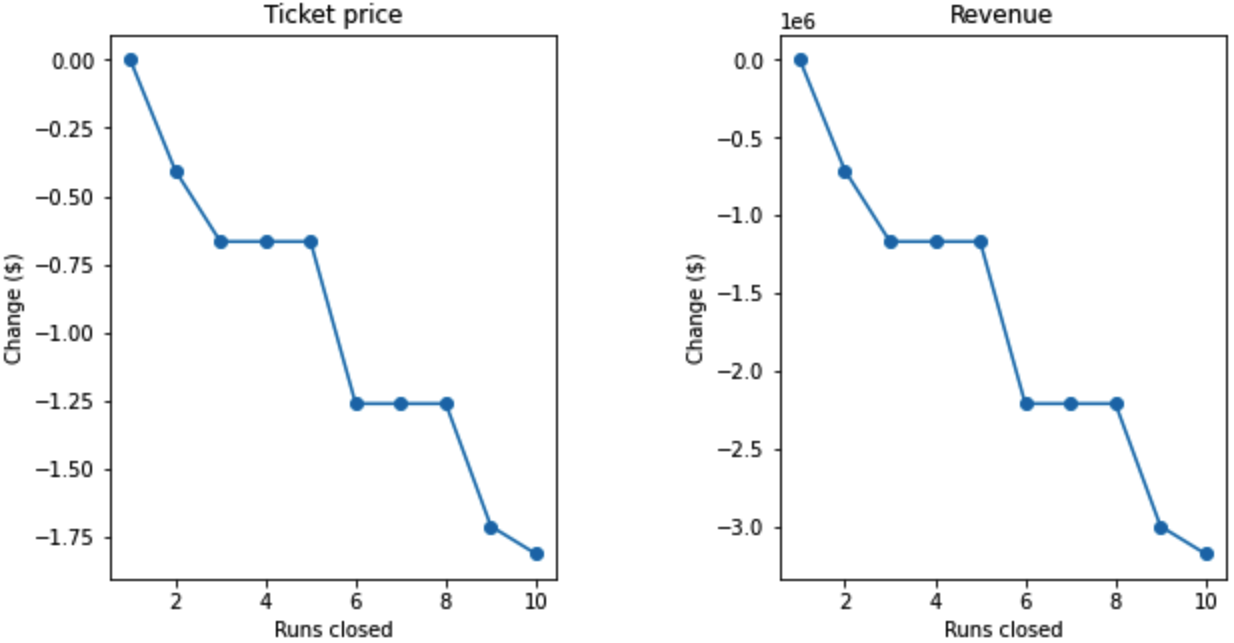
\includegraphics[scale=0.2]{effectofclosingrunsonmarketpriceandrevenue}

From the data, it is not obvious what are the operational costs
associated with features besides chair lifts, but if the reduction in operating
costs from closing runs more than compensates for reduced revenue from a lower
market price for the tickets, it may also be worth it to take into consideration
scenario 1.
\end{frame}

\begin{frame}{Modeling results and analysis}
Scenario 2: increasing the vertical drop by adding a run to a point 150 ft
lower down but requiring the installation of an additional chair lift to
bring skiers back up, without additional snow making coverage
\begin{itemize}
\item This increases the support for the ticket price by \$1.99.
\item Over the season, this is expected to amount to \$3,474,638.
\end{itemize}
Scenario 3: same as scenario 2 but adding 2 acres of snow making cover
\begin{itemize}
\item This increases the support for the ticket price by \$1.99.
\item Over the season, this is expected to amount to \$3,474,638.
\end{itemize}
(no difference from scenario 2)
\end{frame}

\begin{frame}{Modeling results and analysis}
Scenario 4: increase the longest run by 0.2 miles to boast 3.5 miles length,
requiring an additional snow making coverage of 4 acres
\begin{itemize}
\item 
The predicted increase in support for the ticket price in this scenario is zero.
This is expected because the longest run feature has low importance in the
random forest model:
\begin{center}
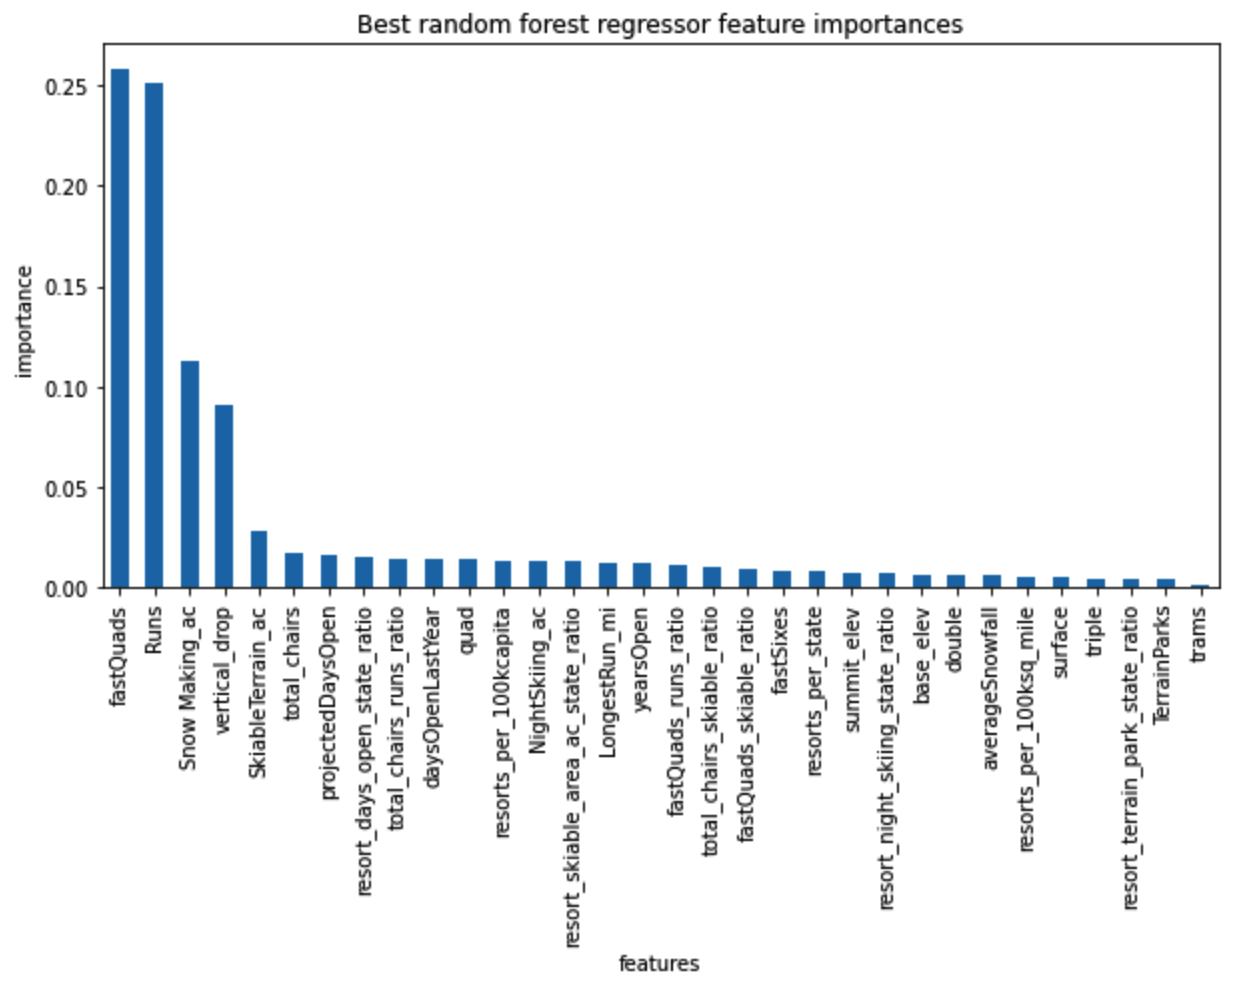
\includegraphics[scale=0.15]{bestrandomforestregressorfeatureimportances}
\end{center}
\end{itemize}
\end{frame}

\begin{frame}{Summary and conclusion}
\begin{itemize}
\item Big Mountain currently charges $\$81$ for an AdultWeekend ticket.
According to my modelling, a ticket price of $\$95.87$ could be
supported in the marketplace by Big Mountain's facilities.

\item The additional operating cost of the new chair lift is $\$1,540,000$, but
per ticket it seems to be less than $\$1$ because installing it, opening a new
run, and increasing the vertical drop by 150 feet supports a price increase of
$\$1.99$ that would account for an increase of revenue of $\$3,474,638$.
I would strongly recommend scenario 2 for further consideration.

\item Scenario 1 could possibly work if the reduction in operating costs from
closing runs more than compensates for reduced revenue from a lower ticket
price.
\end{itemize}
\end{frame}
\end{document}
